% Chapter 14 (English edition) -- ED-22: towards a machine-checked Sandier--Serfaty certificate, 4 steps out of 12 in the Lean kernel
% Translated from papers/discovery_journal_2026/chapters/c14.tex. Figure: code/fig14.py.
\chapter[Four floors out of twelve]{Four floors out of twelve, and the price of the rest}

\reference{Published on 26 October 2026. doi:10.5281/zenodo.23656804}

\section*{The idea in one picture}

A first piece of work (doi:10.5281/\allowbreak zenodo.23653827) reran the program that goes with
the claimed proof of the Sandier--Serfaty conjecture. But rerunning a program is still trusting
it. The next step is to ask the judge, the Lean kernel, to redo the calculations itself,
operation by operation, without going through the program. The title of the paper states the
result up front: it is a \emph{partial} formalisation, and \textbf{the conjecture is not
formally proved; nothing here says that it is.}

\begin{analogie}
A twelve-storey building was put up by a company that nobody has inspected. We rebuild four
storeys to code, under an inspector's eye, and we time what the other eight would cost.
\emph{Where the picture stops:} the storeys are not all the same size. The four redone represent
$0.136\,\%$ of the computational work; two of them rest on one storey (a big table of values)
taken as given, not rebuilt; and even a fully rebuilt building would only say ``the program
computed what it says it computed'', not that its numbers are the right mathematical quantities.
\end{analogie}

\section*{What was done}

The certificate splits into twelve steps. The paper distinguishes two levels of checking. At the
first, the Lean kernel redoes the interval computation of a step and finds, bit for bit, the
integers printed by the original program. At the second, more demanding one, Lean proves that a
true real number, for instance $\pi$, really lies in the announced interval.

Result: four steps out of twelve are complete at the first level (the constants, a boundary
value, the numbers $\lambda$ and $\mu$, and the number $K$), two of them subject to the big table
being taken as given and one subject to coefficients computed elsewhere; only one, that of the
constants, is also complete at the second level. Together, they redo $1{,}685{,}129$ of the
$1{,}238{,}829{,}689$ operations of the original computation. In addition, one lemma from the
``reasoning'' part of the claimed proof is proved entirely in Lean, but for an abstract
function, with no link yet to the certificate.

The rest was costed. Redoing the missing steps at the first level would take on the order of 854
to 2,240 hours of computing on a single processor core, an estimate measured on a busy machine
whose lower end is not a safe bound. The second level for the whole analysis would be a project
of several months.

\begin{encadre}
\textbf{To do with a pencil: what the ``constants'' step computes.} The program obtains $\pi$ from
a classical formula:
$\pi=16\arctan\tfrac15-4\arctan\tfrac1{239}$, with
$\arctan x=x-\tfrac{x^3}{3}+\tfrac{x^5}{5}-\cdots$
With two terms for the first arctangent and one for the second:
$16\,(0.2-0.002667)-4\times0.004184\approx3.157333-0.016736=3.140597$.
Add the next term, $16\times\tfrac{1}{15{,}625}=0.001024$, and you get $3.141621$, already
within $3\times10^{-5}$ of $\pi$. The program takes 150 terms of each series and widens the
interval to cover the remainder; Lean redoes these sums, then proves from its library that the
true $\pi$ is inside.

\textbf{And the share of the work:} $1{,}685{,}129\div1{,}238{,}829{,}689\approx0.00136$, that is
$0.136\,\%$.
\end{encadre}

\section*{How we made sure it is not wrong}

The four steps are \niveau{A} \emph{The judge has looked}: checked by the kernel, axioms within
the short list, without the shortcut that would trust the compiler, and a replay of these modules
by the kernel, on 26 October, passed without error. Eleven false claims were planted on purpose,
for example $\log 2$ computed with 199 terms instead of 200, or an error margin divided by 12
instead of 24; all are rejected.

A separate auditor agent rebuilt thirteen modules from the sources, in its own folder: the files
obtained are identical byte for byte. It compared the Lean transcription with the original
program line by line, and checked with a script that the 18,455 table values copied into Lean are
indeed those of the program (a difference of one unit in the last digit would otherwise go
unnoticed). Verdict: ``accept with corrections'', with two text corrections, including one claim
that was too broad (a check of the original program was not covered). No human has read this
work.

\section*{What this does not say}

\begin{limite}
\begin{itemize}
\item \textbf{The conjecture is not proved}, neither formally nor otherwise; everything remains
  conditional on the manuscript produced by an AI.
\item Eight steps out of twelve are not complete at the first level, and they are the ones that
  carry most of the analysis; the amount of computing work is not the content of the proof.
\item Two redone steps depend on the big table, taken as given.
\item One reasoning step out of thirty-one is complete in Lean, plus the algebraic part of a
  second.
\end{itemize}
\end{limite}

The progress is announced as a fraction, not as a victory. That is precisely what makes it
usable: everyone knows what is left to do, and how much it would cost.

\section*{Going further}

The paper (10 pages), with the table of the twelve steps and the quote for the rest:
doi:10.5281/\allowbreak zenodo.23656804. It follows doi:10.5281/\allowbreak zenodo.23653827.

\begin{figure}[ht]
\centering
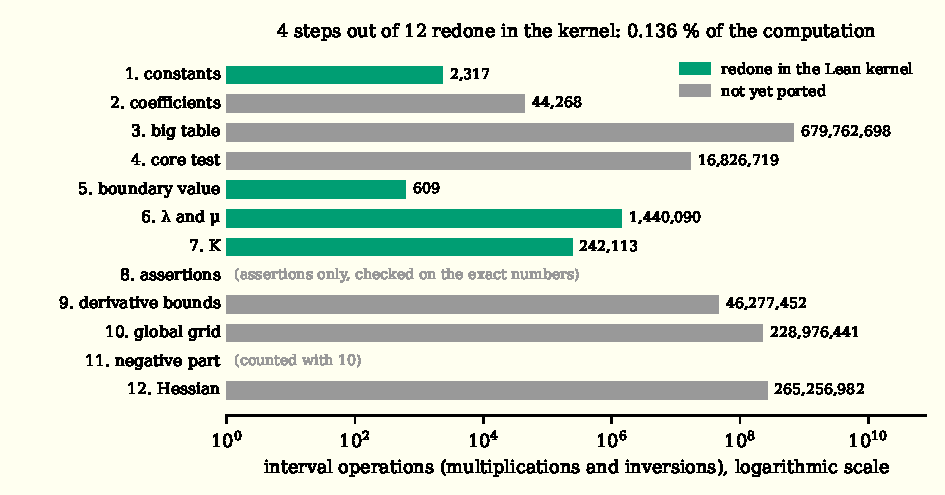
\includegraphics[width=\linewidth]{figures/c14_etapes}
\caption{The twelve steps of the certificate, by number of operations; in green, those that the Lean kernel redid.}
\end{figure}
